% ============================================================================
% FL-TTA-IoT-IDS: Methodology Flow Diagrams (XeLaTeX, A4, Single Column)
% Each page = One sequential part of the methodology pipeline
% ============================================================================
\documentclass[a4paper,12pt]{article}

% XeLaTeX font setup
\usepackage{fontspec}
\setmainfont{Times New Roman}

% Page geometry - A4 with safe margins
\usepackage[a4paper, margin=2cm, top=2.5cm, bottom=2.5cm]{geometry}

% Graphics and TikZ
\usepackage{graphicx}
\usepackage{tikz}
\usetikzlibrary{shapes.geometric, arrows.meta, positioning, calc, fit, backgrounds, decorations.pathreplacing}

% Colors - Professional palette
\definecolor{datacolor}{RGB}{52, 152, 219}      % Blue - Data/Input
\definecolor{processcolor}{RGB}{46, 204, 113}   % Green - Processing
\definecolor{flcolor}{RGB}{231, 76, 60}         % Red - Federated Learning
\definecolor{ttacolor}{RGB}{241, 196, 15}       % Yellow - TTA
\definecolor{outputcolor}{RGB}{155, 89, 182}    % Purple - Output
\definecolor{servercolor}{RGB}{52, 73, 94}      % Dark - Server
\definecolor{clientcolor}{RGB}{230, 126, 34}    % Orange - Client
\definecolor{arrowcolor}{RGB}{44, 62, 80}       % Dark gray - Arrows

% TikZ styles
\tikzset{
    % Base styles
    basenode/.style={
        draw, thick, align=center, font=\small,
        minimum width=4.5cm, minimum height=1.2cm,
        rounded corners=3pt
    },
    % Specific node types
    datanode/.style={basenode, fill=datacolor!20, draw=datacolor!70},
    processnode/.style={basenode, fill=processcolor!20, draw=processcolor!70},
    flnode/.style={basenode, fill=flcolor!20, draw=flcolor!70},
    ttanode/.style={basenode, fill=ttacolor!20, draw=ttacolor!70},
    outputnode/.style={basenode, fill=outputcolor!20, draw=outputcolor!70},
    servernode/.style={basenode, fill=servercolor!15, draw=servercolor!70},
    clientnode/.style={basenode, fill=clientcolor!20, draw=clientcolor!70, minimum width=3.2cm},
    % Decision diamond
    decision/.style={
        diamond, draw, thick, align=center, font=\small,
        minimum width=2.5cm, minimum height=2cm,
        fill=ttacolor!25, draw=ttacolor!70,
        aspect=2
    },
    % Arrows
    myarrow/.style={-{Stealth[length=3mm]}, thick, arrowcolor},
    dashedarrow/.style={-{Stealth[length=3mm]}, thick, arrowcolor, dashed},
    % Labels
    steplabel/.style={font=\footnotesize\itshape, text=gray},
    eqlabel/.style={font=\scriptsize, text=black!70},
    % Grouping box
    groupbox/.style={draw=gray, dashed, rounded corners=5pt, inner sep=8pt},
}

% No paragraph indent
\setlength{\parindent}{0pt}

% Headers
\usepackage{fancyhdr}
\pagestyle{fancy}
\fancyhf{}
\fancyhead[L]{\small\textit{FL-TTA-IoT-IDS Methodology}}
\fancyhead[R]{\small Page \thepage\ of 4}
\renewcommand{\headrulewidth}{0.4pt}

\begin{document}

% ============================================================================
% PAGE 1: Data Collection and Preprocessing
% ============================================================================
\begin{center}
\textbf{\Large Part 1: IoT-23 Data Collection \& Preprocessing}
\end{center}
\vspace{0.5cm}

\begin{center}
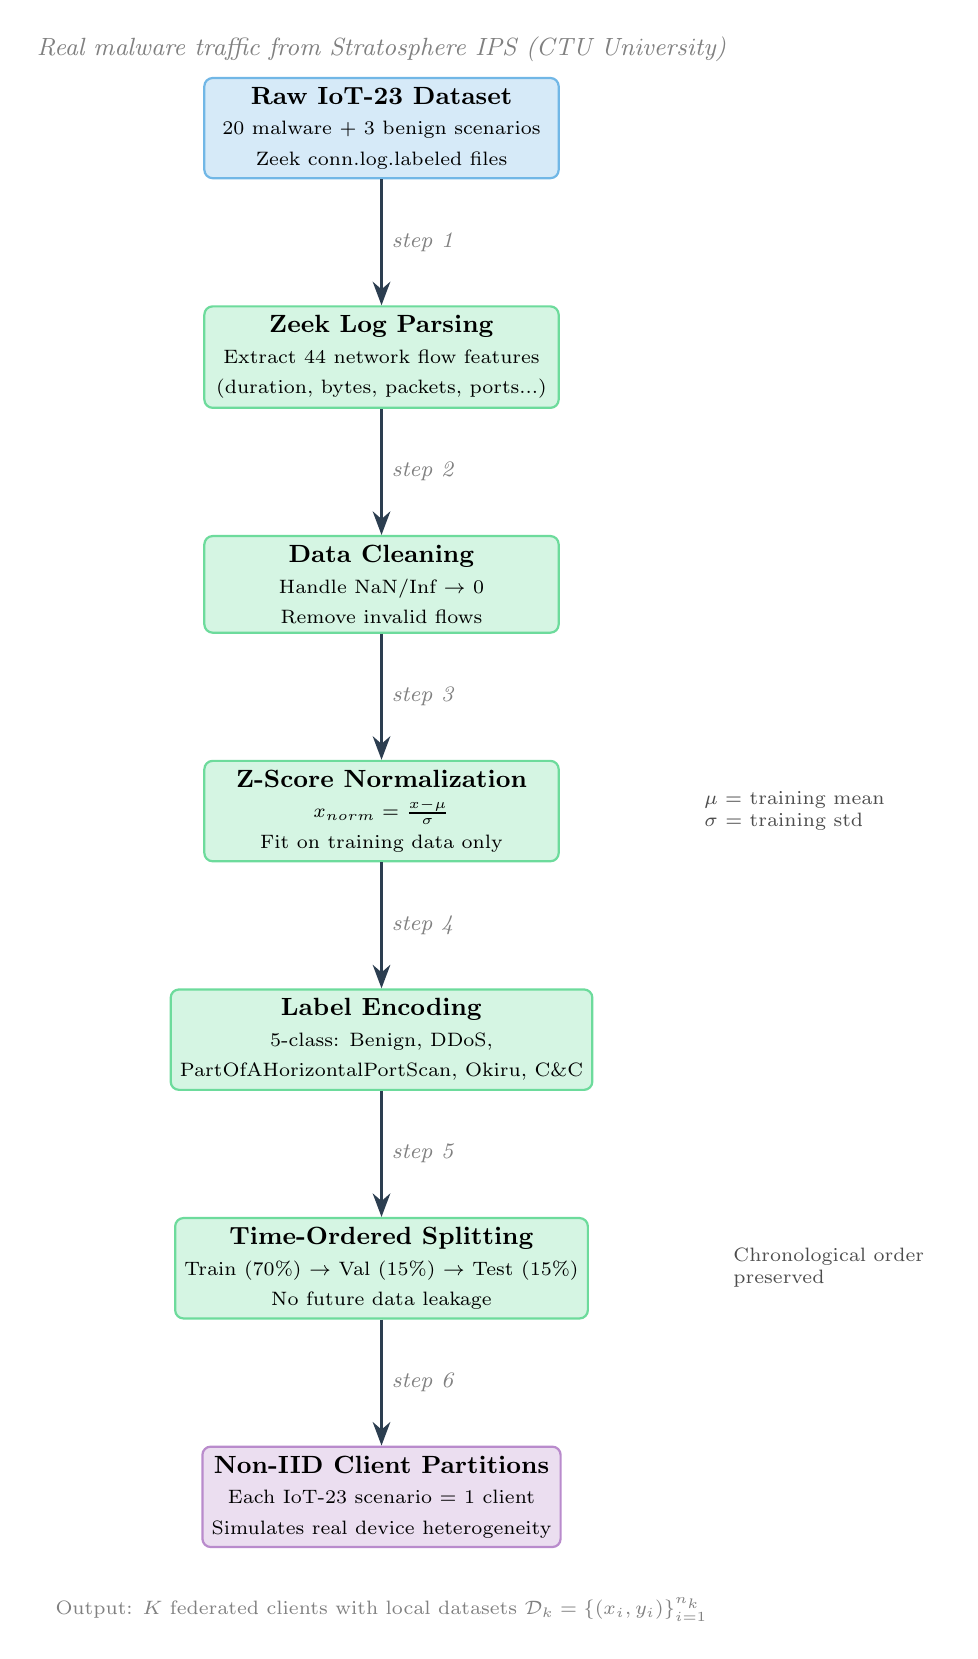
\begin{tikzpicture}[node distance=1.6cm]

% Title annotation
\node[font=\small\itshape, text=gray] at (0, 1) {Real malware traffic from Stratosphere IPS (CTU University)};

% Nodes
\node (raw) [datanode] {
    \textbf{Raw IoT-23 Dataset}\\
    \scriptsize 20 malware + 3 benign scenarios\\
    \scriptsize Zeek conn.log.labeled files
};

\node (parse) [processnode, below=of raw] {
    \textbf{Zeek Log Parsing}\\
    \scriptsize Extract 44 network flow features\\
    \scriptsize (duration, bytes, packets, ports...)
};

\node (clean) [processnode, below=of parse] {
    \textbf{Data Cleaning}\\
    \scriptsize Handle NaN/Inf $\rightarrow$ 0\\
    \scriptsize Remove invalid flows
};

\node (normalize) [processnode, below=of clean] {
    \textbf{Z-Score Normalization}\\
    \scriptsize $x_{norm} = \frac{x - \mu}{\sigma}$\\
    \scriptsize Fit on training data only
};

\node (label) [processnode, below=of normalize] {
    \textbf{Label Encoding}\\
    \scriptsize 5-class: Benign, DDoS,\\
    \scriptsize PartOfAHorizontalPortScan, Okiru, C\&C
};

\node (split) [processnode, below=of label] {
    \textbf{Time-Ordered Splitting}\\
    \scriptsize Train (70\%) $\rightarrow$ Val (15\%) $\rightarrow$ Test (15\%)\\
    \scriptsize No future data leakage
};

\node (clients) [outputnode, below=of split] {
    \textbf{Non-IID Client Partitions}\\
    \scriptsize Each IoT-23 scenario = 1 client\\
    \scriptsize Simulates real device heterogeneity
};

% Arrows with step labels
\draw[myarrow] (raw) -- (parse) node[midway, right, steplabel] {step 1};
\draw[myarrow] (parse) -- (clean) node[midway, right, steplabel] {step 2};
\draw[myarrow] (clean) -- (normalize) node[midway, right, steplabel] {step 3};
\draw[myarrow] (normalize) -- (label) node[midway, right, steplabel] {step 4};
\draw[myarrow] (label) -- (split) node[midway, right, steplabel] {step 5};
\draw[myarrow] (split) -- (clients) node[midway, right, steplabel] {step 6};

% Side annotations
\node[eqlabel, right=1.5cm of normalize] {
    \begin{tabular}{l}
    $\mu$ = training mean\\
    $\sigma$ = training std
    \end{tabular}
};

\node[eqlabel, right=1.5cm of split] {
    \begin{tabular}{l}
    Chronological order\\
    preserved
    \end{tabular}
};

% Bottom annotation
\node[font=\scriptsize, text=gray, below=0.5cm of clients] {
    Output: $K$ federated clients with local datasets $\mathcal{D}_k = \{(x_i, y_i)\}_{i=1}^{n_k}$
};

\end{tikzpicture}
\end{center}

\newpage

% ============================================================================
% PAGE 2: Federated Learning Training
% ============================================================================
\begin{center}
\textbf{\Large Part 2: Federated Learning Training (FedAvg/FedProx)}
\end{center}
\vspace{0.3cm}

\begin{center}
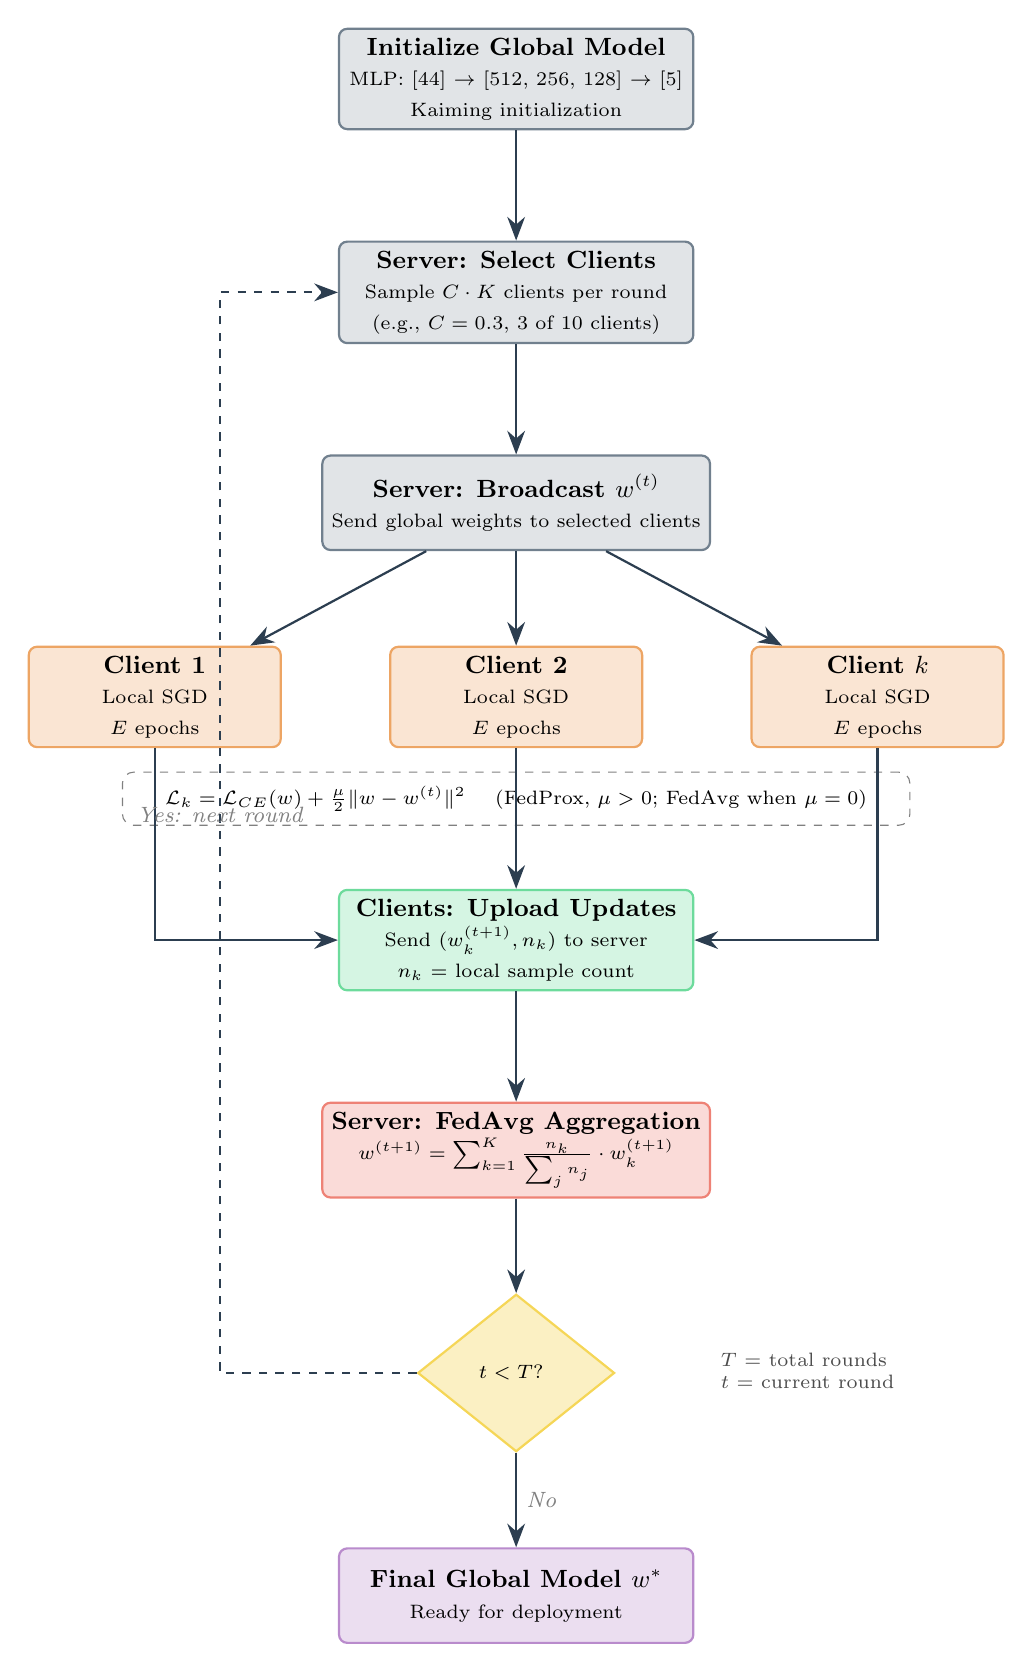
\begin{tikzpicture}[node distance=1.4cm]

% Server section
\node (init) [servernode] {
    \textbf{Initialize Global Model}\\
    \scriptsize MLP: [44] $\rightarrow$ [512, 256, 128] $\rightarrow$ [5]\\
    \scriptsize Kaiming initialization
};

\node (select) [servernode, below=of init] {
    \textbf{Server: Select Clients}\\
    \scriptsize Sample $C \cdot K$ clients per round\\
    \scriptsize (e.g., $C=0.3$, 3 of 10 clients)
};

\node (broadcast) [servernode, below=of select] {
    \textbf{Server: Broadcast $w^{(t)}$}\\
    \scriptsize Send global weights to selected clients
};

% Client training (side by side)
\node (client1) [clientnode, below left=1.2cm and 0.5cm of broadcast] {
    \textbf{Client 1}\\
    \scriptsize Local SGD\\
    \scriptsize $E$ epochs
};

\node (client2) [clientnode, below=1.2cm of broadcast] {
    \textbf{Client 2}\\
    \scriptsize Local SGD\\
    \scriptsize $E$ epochs
};

\node (client3) [clientnode, below right=1.2cm and 0.5cm of broadcast] {
    \textbf{Client $k$}\\
    \scriptsize Local SGD\\
    \scriptsize $E$ epochs
};

% Loss function annotation
\node (lossbox) [draw=gray, dashed, rounded corners, inner sep=5pt, below=2.8cm of broadcast, minimum width=10cm] {
    \scriptsize $\mathcal{L}_k = \mathcal{L}_{CE}(w) + \frac{\mu}{2}\|w - w^{(t)}\|^2$ \quad (FedProx, $\mu > 0$; FedAvg when $\mu = 0$)
};

% Upload
\node (upload) [processnode, below=0.8cm of lossbox] {
    \textbf{Clients: Upload Updates}\\
    \scriptsize Send $(w_k^{(t+1)}, n_k)$ to server\\
    \scriptsize $n_k$ = local sample count
};

% Aggregation
\node (aggregate) [flnode, below=of upload] {
    \textbf{Server: FedAvg Aggregation}\\
    \scriptsize $w^{(t+1)} = \sum_{k=1}^{K} \frac{n_k}{\sum_j n_j} \cdot w_k^{(t+1)}$
};

% Check convergence
\node (check) [decision, below=1.2cm of aggregate] {
    \scriptsize $t < T$?
};

% Output
\node (globalmodel) [outputnode, below=1.2cm of check] {
    \textbf{Final Global Model $w^*$}\\
    \scriptsize Ready for deployment
};

% Arrows
\draw[myarrow] (init) -- (select);
\draw[myarrow] (select) -- (broadcast);
\draw[myarrow] (broadcast) -- (client1);
\draw[myarrow] (broadcast) -- (client2);
\draw[myarrow] (broadcast) -- (client3);
\draw[myarrow] (client1) |- (upload);
\draw[myarrow] (client2) -- (upload);
\draw[myarrow] (client3) |- (upload);
\draw[myarrow] (upload) -- (aggregate);
\draw[myarrow] (aggregate) -- (check);
\draw[myarrow] (check) -- node[right, steplabel] {No} (globalmodel);
\draw[dashedarrow] (check.west) -- ++(-2.5,0) |- (select.west) node[pos=0.25, above, steplabel] {Yes: next round};

% Round counter annotation
\node[eqlabel, right=1cm of check] {
    \begin{tabular}{l}
    $T$ = total rounds\\
    $t$ = current round
    \end{tabular}
};

\end{tikzpicture}
\end{center}

\newpage

% ============================================================================
% PAGE 3: Drift-Aware Test-Time Adaptation
% ============================================================================
\begin{center}
\textbf{\Large Part 3: Drift-Aware Test-Time Adaptation (TTA)}
\end{center}
\vspace{0.3cm}

\begin{center}
\begin{tikzpicture}[node distance=1.3cm]

% Input
\node (deploy) [datanode] {
    \textbf{Deployed Global Model $w^*$}\\
    \scriptsize From federated training (Part 2)
};

\node (stream) [datanode, below=of deploy] {
    \textbf{Incoming Test Batch $\mathcal{B}_t$}\\
    \scriptsize Live IoT traffic (unlabeled)
};

% Forward pass
\node (forward) [processnode, below=of stream] {
    \textbf{Forward Pass}\\
    \scriptsize $z = f_{w}(x)$, \quad $p = \text{softmax}(z)$
};

% Entropy computation
\node (entropy) [ttanode, below=of forward] {
    \textbf{Compute Batch Entropy}\\
    \scriptsize $H(p) = -\sum_{c=1}^{C} p_c \log p_c$\\
    \scriptsize $\bar{H}_t = \frac{1}{B}\sum_{i=1}^{B} H(p_i)$
};

% Drift check
\node (driftcheck) [decision, below=1.4cm of entropy] {
    \scriptsize Drift?
};

% Drift condition annotation
\node[eqlabel, right=2cm of driftcheck] {
    \begin{tabular}{l}
    Drift if:\\[2pt]
    $\dfrac{\bar{H}_t - \bar{H}_{base}}{\bar{H}_{base}} > \delta$\\[4pt]
    ($\delta = 0.3$ default)
    \end{tabular}
};

% No drift path
\node (nodrift) [outputnode, below left=1.5cm and 1cm of driftcheck] {
    \textbf{Standard Prediction}\\
    \scriptsize $\hat{y} = \arg\max_c p_c$\\
    \scriptsize No model update
};

% Yes drift path - reliability filter
\node (filter) [ttanode, below right=1.5cm and 1cm of driftcheck] {
    \textbf{Reliability Filter (EATA)}\\
    \scriptsize Keep samples where\\
    \scriptsize $H(p_i) < \tau$ \quad ($\tau = 0.4 \ln 2$)
};

% TTA update
\node (ttaupdate) [flnode, below=of filter] {
    \textbf{TTA: Entropy Minimization}\\
    \scriptsize Update BatchNorm params only:\\
    \scriptsize $\theta \leftarrow \theta - \eta \nabla_\theta \bar{H}_{reliable}$
};

% Anti-forgetting
\node (fisher) [processnode, below=of ttaupdate] {
    \textbf{Anti-Forgetting (Optional)}\\
    \scriptsize $\mathcal{L} = \bar{H} + \alpha \sum_k F_k(w_k - w_k^{anchor})^2$\\
    \scriptsize Fisher regularization
};

% Final output
\node (finalout) [outputnode, below=1.2cm of nodrift, xshift=2cm] {
    \textbf{Final Prediction}\\
    \scriptsize 5-class: Benign, DDoS, Scan, Okiru, C\&C
};

% Arrows
\draw[myarrow] (deploy) -- (stream);
\draw[myarrow] (stream) -- (forward);
\draw[myarrow] (forward) -- (entropy);
\draw[myarrow] (entropy) -- (driftcheck);
\draw[myarrow] (driftcheck) -- node[above, steplabel] {No} (nodrift);
\draw[myarrow] (driftcheck) -- node[above, steplabel] {Yes} (filter);
\draw[myarrow] (filter) -- (ttaupdate);
\draw[myarrow] (ttaupdate) -- (fisher);
\draw[myarrow] (nodrift) -- (finalout);
\draw[myarrow] (fisher) |- (finalout);

% Feedback loop
\draw[dashedarrow] (fisher.west) -- ++(-3.5,0) |- (forward.west) node[pos=0.15, left, steplabel] {Updated model};

\end{tikzpicture}
\end{center}

\newpage

% ============================================================================
% PAGE 4: Complete End-to-End System Overview
% ============================================================================
\begin{center}
\textbf{\Large Part 4: Complete FL-TTA-IoT-IDS System Overview}
\end{center}
\vspace{0.2cm}

\begin{center}
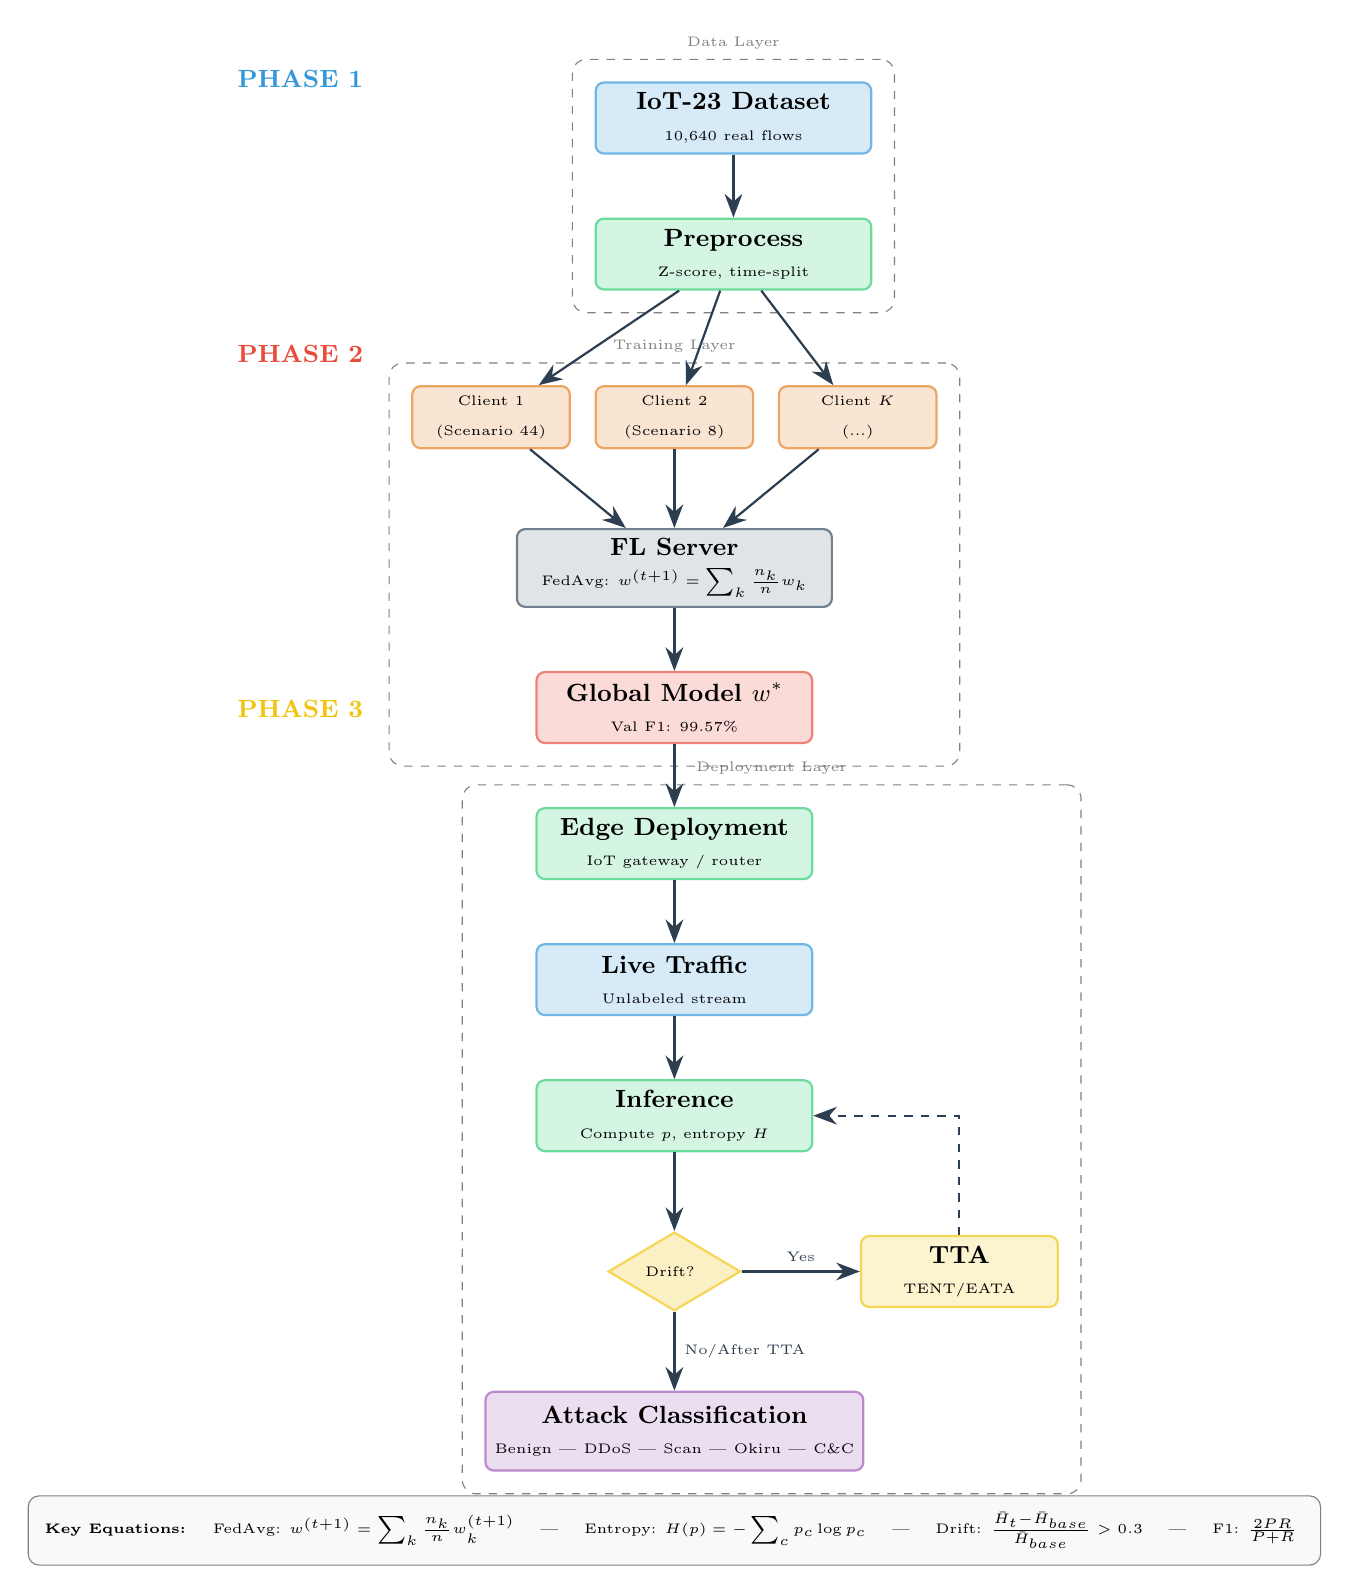
\begin{tikzpicture}[node distance=1.1cm, every node/.style={font=\scriptsize}]

% ===== PHASE 1: Data =====
\node[font=\small\bfseries, text=datacolor] at (-5.5, 0.5) {PHASE 1};
\node (iot23) [datanode, minimum width=3.5cm, minimum height=0.9cm] {
    \textbf{IoT-23 Dataset}\\
    \tiny 10,640 real flows
};

\node (preprocess) [processnode, below=0.8cm of iot23, minimum width=3.5cm, minimum height=0.9cm] {
    \textbf{Preprocess}\\
    \tiny Z-score, time-split
};

\draw[myarrow] (iot23) -- (preprocess);

% ===== PHASE 2: FL Training =====
\node[font=\small\bfseries, text=flcolor] at (-5.5, -3) {PHASE 2};

% Clients
\node (c1) [clientnode, below left=1.2cm and 0.3cm of preprocess, minimum width=2cm, minimum height=0.7cm] {
    \tiny Client 1\\
    \tiny (Scenario 44)
};
\node (c2) [clientnode, right=0.3cm of c1, minimum width=2cm, minimum height=0.7cm] {
    \tiny Client 2\\
    \tiny (Scenario 8)
};
\node (ck) [clientnode, right=0.3cm of c2, minimum width=2cm, minimum height=0.7cm] {
    \tiny Client $K$\\
    \tiny (...)
};

\draw[myarrow] (preprocess) -- (c1);
\draw[myarrow] (preprocess) -- (c2);
\draw[myarrow] (preprocess) -- (ck);

% Server
\node (server) [servernode, below=1cm of c2, minimum width=4cm, minimum height=0.9cm] {
    \textbf{FL Server}\\
    \tiny FedAvg: $w^{(t+1)} = \sum_k \frac{n_k}{n} w_k$
};

\draw[myarrow] (c1) -- (server);
\draw[myarrow] (c2) -- (server);
\draw[myarrow] (ck) -- (server);

% Global model
\node (global) [flnode, below=0.8cm of server, minimum width=3.5cm, minimum height=0.9cm] {
    \textbf{Global Model $w^*$}\\
    \tiny Val F1: 99.57\%
};

\draw[myarrow] (server) -- (global);

% ===== PHASE 3: Deployment + TTA =====
\node[font=\small\bfseries, text=ttacolor] at (-5.5, -7.5) {PHASE 3};

\node (edge) [processnode, below=0.8cm of global, minimum width=3.5cm, minimum height=0.9cm] {
    \textbf{Edge Deployment}\\
    \tiny IoT gateway / router
};

\draw[myarrow] (global) -- (edge);

\node (live) [datanode, below=0.8cm of edge, minimum width=3.5cm, minimum height=0.9cm] {
    \textbf{Live Traffic}\\
    \tiny Unlabeled stream
};

\draw[myarrow] (edge) -- (live);

% Inference + drift check
\node (infer) [processnode, below=0.8cm of live, minimum width=3.5cm, minimum height=0.9cm] {
    \textbf{Inference}\\
    \tiny Compute $p$, entropy $H$
};

\draw[myarrow] (live) -- (infer);

% Decision
\node (drift) [decision, below=1cm of infer, minimum width=1.5cm, minimum height=1cm] {
    \tiny Drift?
};

\draw[myarrow] (infer) -- (drift);

% TTA path
\node (tta) [ttanode, right=1.5cm of drift, minimum width=2.5cm, minimum height=0.9cm] {
    \textbf{TTA}\\
    \tiny TENT/EATA
};

\draw[myarrow] (drift) -- node[above, font=\tiny] {Yes} (tta);
\draw[dashedarrow] (tta) |- (infer);

% Output
\node (output) [outputnode, below=1cm of drift, minimum width=4cm, minimum height=1cm] {
    \textbf{Attack Classification}\\
    \tiny Benign | DDoS | Scan | Okiru | C\&C
};

\draw[myarrow] (drift) -- node[right, font=\tiny] {No/After TTA} (output);

% ===== Phase labels on side =====
\begin{scope}[on background layer]
    \node[groupbox, fit=(iot23)(preprocess), label={[font=\tiny, text=gray]above:Data Layer}] {};
    \node[groupbox, fit=(c1)(c2)(ck)(server)(global), label={[font=\tiny, text=gray]above:Training Layer}] {};
    \node[groupbox, fit=(edge)(live)(infer)(drift)(tta)(output), label={[font=\tiny, text=gray]above:Deployment Layer}] {};
\end{scope}

% Key equations summary box
\node[draw=gray, fill=gray!5, rounded corners, inner sep=6pt, 
      below=0.3cm of output, minimum width=12cm, align=left, font=\tiny] {
    \textbf{Key Equations:} \quad
    FedAvg: $w^{(t+1)} = \sum_{k} \frac{n_k}{n} w_k^{(t+1)}$ \quad | \quad
    Entropy: $H(p) = -\sum_c p_c \log p_c$ \quad | \quad
    Drift: $\frac{\bar{H}_t - \bar{H}_{base}}{\bar{H}_{base}} > 0.3$ \quad | \quad
    F1: $\frac{2PR}{P+R}$
};

\end{tikzpicture}
\end{center}

\end{document}
